\documentclass[a4paper]{article}
\usepackage[left=3cm,right=3cm,top=2cm,bottom=2cm]{geometry} % page settings
\usepackage{enumerate}
\usepackage{hyperref}
\usepackage{graphicx}
\usepackage{amsfonts}
\usepackage{amsthm}
\usepackage{mathtools}
\usepackage{titlesec}
\usepackage{polski}
\usepackage{tikz}
\usepackage[utf8]{inputenc}
\DeclarePairedDelimiter\ceil{\lceil}{\rceil}
\DeclarePairedDelimiter\floor{\lfloor}{\rfloor}

\def\checkmark{\tikz\fill[scale=0.3](0,.35) -- (.25,0) -- (1,.7) -- (.25,.15) -- cycle;} 

\titlespacing*{\subsection}
{0ex}{10ex}{3ex}

\title{Lista 11}
\author{Kamil Matuszewski}
\date{\today}

\begin{document}

\maketitle
\setlength{\parindent}{0.5ex}
\setlength{\parskip}{1.5ex}
\newcommand{\R}{\mathbb{R}}

\begin{center}
\begin{tabular}{|c *{8}{|c} |c|}\hline
1 & 2 & 3 & 4 & 5 & 6 & 7 & 8\\
\hline 
\checkmark &\checkmark &\checkmark &\checkmark & &\checkmark &\checkmark &\checkmark\\
\hline
\end{tabular}\\
\end{center}

\subsection*{Zadanie 1}
Uzasadnij proces ortogonalizacji Grama-Schmidta.

Na początek, jak działa ortogonalizacja Grama-Schmidta:
Dla układu liniowo niezależnego $\lbrace f_0,f_1,\cdots , f_n \rbrace$ możemy utworzyć układ liniowo niezależny $\lbrace g_0,g_1,\cdots , g_n \rbrace$ taki, że $<g_i,g_j>_N=0$ dla $i \neq j$, za pomocą następującego algorytmu:  
$$\begin{matrix*}[l]
g_0=f_0\\
g_k=f_k-\sum\limits_{j=0}^{k-1}\frac{<f_k,g_j>}{<g_j,g_j>}g_j
\end{matrix*}$$
Muszę najpierw udowodnić, że tak otrzymany układ jest ortogonalny.
\begin{proof}
Indukcja. Niech $g_0\cdots g_k$ będzie układem wektorów uzyskanym za pomocą tego algorytmu z bazy $v_0\cdots v_n$. Załóżmy indukcyjnie, że $g_0\cdots g_{k-1}$ są ortogonalne. Sprawdzę ortogonalność $g_k$ względem dowolnego $g_i$ gdzie $i<k$.\\
Zapiszmy $g_k$ jako:\\
$$g_k=f_k-\sum\limits_{j=0}^{k-1}\frac{<f_k,g_j>}{<g_j,g_j>}g_j $$
Korzystając z własności iloczynu skalarnego, mamy:\\
$$<g_i,g_k>=\left< g_i,f_k-\sum\limits_{j=0}^{k-1}\frac{<f_k,g_j>}{<g_j,g_j>}g_j\right>$$
$$<g_i,g_k>=<g_i,f_k>-\sum\limits_{j=0}^{k-1}\frac{<f_k,g_j>}{<g_j,g_j>}<g_j,g_i>$$

Z założenia indukcyjnego, wiemy, że $<g_j,g_i>=0$ dla $j\neq i$, więc zostaje nam:
$$<g_i,g_k>=<g_i,f_k>-\frac{<f_k,g_i>}{<g_i,g_i>}<g_i,g_i>$$
$$<g_i,g_k>=<g_i,f_k>-<f_k,g_i>$$
$$<g_i,g_k>=0$$
Co oznacza, że $g_k$ jest ortogonalny z dowolnym $g_i$.


\end{proof}

\subsection*{Zadanie 2}
Układ ortogonalny $\lbrace P_0,P_1,\cdots ,P_n \rbrace$ jest bazą $\prod_n $
\begin{proof}
Skoro tych wielomianów jest $n+1$, to wystarczy sprawdzić liniową niezależność.
$$\alpha_0 P_0+\alpha_1 P_1+\cdots+\alpha_n P_n=0 $$
Pomnóżmy (w sensie iloczynu skalarnego) przez $P_i$ (gdzie $i$ jest dowolne).
$$\begin{matrix*}[l]
\alpha_0 P_0+\alpha_1 P_1+\cdots+\alpha_n P_n=0 &&& \backslash \cdot P_i\\
\alpha_0 <P_0,P_i>+\alpha_1 <P_1,P_i>+\cdots + \alpha_i <P_i,P_i> +\cdots +\alpha_n <P_n,P_i>=0
\end{matrix*} $$
Teraz, wiemy, że dla każdego $j\neq i$ $<P_i,P_j>=0$ (bo są ortogonalne), więc:
$$\alpha_i <P_i,P_i> = 0$$
$$\alpha_i = 0$$
Skoro możemy to zrobić dla każdego $i$, możemy napisać, że:
$$\alpha_0+\alpha_1+\cdots +\alpha_i = 0$$
A to jest to co chcieliśmy pokazać.
\end{proof}

\subsection*{Zadanie 3}
Zapiszmy $w \in \prod_{k-1}$ jako kombinację liniową $P_0...P_{k-1}$, Iloczyn sumy to suma iloczynów, każdy z iloczynów jest 0, więc wszystko jest 0.
$$<a_0P_0P_k,a_1P_1P_k,\dots ,a_{k-1}P_{k-1}P_{k}> = <0,0,\dots ,0>=0$$
Bo $<P_i,P_k>=0$ z ortogonalności.

\subsection*{Zadanie 4}
Pokaż, że wielomiany Czebyszewa są ortogonalne względem iloczynu skalarnego w postaci $$\sum\limits_{k=0}^{r} p_kf(u_k)g(u_k),$$ gdzie $u_k=\cos(\frac{k\pi}{r})$ $(k=0\dots r)$ oraz $$p(u_k) = \left\{\begin{matrix}
\frac{1}{2} & (k=0,r), \\ 
1 & (1<k<r) 
\end{matrix}\right.$$

Najpierw pokażę taki wzórek:
$$\sum\limits_{k=0}^{r} cos(k\alpha) = \frac{1}{2}+\frac{\sin((N+\frac{1}{2})\alpha)}{2\sin(\frac{\alpha}{2})} $$
$$(1) \sum\limits_{k=0}^{r}{}^{'} cos(k\alpha) = \frac{\sin((N+\frac{1}{2})\alpha)}{2\sin(\frac{\alpha}{2})} $$
\begin{proof}
Ze stacka, ale fajny i zrozumiały więc wklejam.\\

\includegraphics[scale=0.7]{2.png}


\end{proof}

Teraz, przejdźmy do dowodu właściwego.

\begin{proof}


Powiem też, że zapis $\sum\limits_{k=0}^{r}{}^{''}$ oznacza sumę z połowionym pierwszym i ostatnim wyrazem(uproszczenie zapisu).
Teraz, policzmy iloczyn skalarny dowolnych dwóch wielomianów Czebyszewa.
$$<T_a,T_b> = \sum\limits_{k=0}^{r}{}^{''}T_a(u_k) T_b(u_k)$$
Ale, $u_k \in [-1,1]$ więc $T_a(u_k) = \cos(a \arccos (\cos(\frac{k\pi}{r})))=\cos(a \frac{k\pi}{r}))$ więc,
$$<T_a,T_b> = \sum\limits_{k=0}^{r}{}^{''} \cos(a \frac{k\pi}{r}) \cos(b \frac{k\pi}{r})$$
Ze wzoru na iloczyn cosinusów:
$$\frac{1}{2} \sum\limits_{k=0}^{r}{}^{''} \cos(k(a-b)\frac{\pi}{r}) + \frac{1}{2} \sum\limits_{k=0}^{r}{}^{''} \cos(k(a+b)\frac{\pi}{r})$$
Teraz, z (1), mamy
$$\frac{1}{2} \frac{\sin((r+\frac{1}{2})\frac{(a-b)\pi}{r})}{2\sin{\frac{(a-b)\pi}{2r}}} - \frac{1}{4}\cos((a-b)\pi) + \frac{1}{2} \frac{\sin((r+\frac{1}{2})\frac{(a+b)\pi}{r})}{2\sin{\frac{(a+b)\pi}{2r}}} - \frac{1}{4}\cos((a+b)\pi)$$
Rozpiszmy $\sin(a+b)=\sin(a)\cos(b)+\cos(a)\sin(b)$
$$\frac{1}{2} \frac{\sin((a-b)\pi)\cos(\frac{(a-b)\pi}{2r}) + \sin(\frac{(a-b)\pi}{2r})\cos((a-b)\pi)}{2\sin{\frac{(a-b)\pi}{2r}}} - \frac{1}{4}\cos((a-b)\pi) +$$ $$+ \frac{1}{2} \frac{\sin((a+b)\pi)\cos(\frac{(a+b)\pi}{2r}) + \sin(\frac{(a+b)\pi}{2r})\cos((a+b)\pi)}{2\sin{\frac{(a+b)\pi}{2r}}} - \frac{1}{4}\cos((a+b)\pi)$$
Teraz, $\sin{k\pi}=0$, oraz po skróceniu:
$$\frac{1}{4} \cos((a-b)\pi) - \frac{1}{4}\cos((a-b)\pi) + \frac{1}{4} \cos((a+b)\pi) - \frac{1}{4}\cos((a+b)\pi)=0$$
Czyli $<T_a,T_b>=0$
Czyli są ortogonalne.
\end{proof}


\subsection*{Zadanie 6}
Niech ciąg $\lbrace P_k \rbrace$ będzie określony w sposób:\\
$$
\left\{\begin{matrix}
P_0(x)=1 \\ 
P_1(x)=x-c_1 \\
P_k(x)=(x-c_k)P_{k-1}(x) -d_kP_{k-2}(x) &&&&& (k= 2,3,\dots) 
\end{matrix}\right.
$$


Pokaż, że algorytm:
$$
\begin{matrix*}[l]
B_{m+2}=B_{m+1}=0\\
B_k=a_k+(x-c_{k+1})B_{k+1}-d_{k+2}B_{k+2} &&& (k=m,m-1,\dots , 0)\\
wynik=B_0
\end{matrix*}
$$
Oblicza $\sum\limits_{k=0}^{m}a_kP_k(x)$
\begin{proof}
$$
B_0=a_0+(x-c_1)B_1-d_2B_2=a_0P_0+P_1B_1-d_2B_2=a_0P_0+P_1(a_1+(x-c_2)B_2-d_3B_3)-d_2B_2=$$ $$=a_0P_0+a_1P_1+(P_1(x-c_2)-d_2)B_2-P_1d_3B_3=a_0P_0+a_1P_1+P_2B_2-P_1d_3B_3=$$ $$=a_0P_0+a_1P_1+a_2P_2+((x-c_3)P_2-d_3P_1)B_3-P_2d_4B_4=a_0P_0+a_1P_1+a_2P_2+P_3B_3-P_2d_4B_4=$$ $$=\dots=\sum\limits_{k=0}^{i}a_kP_k(x) + P_{i+1}B_{i+1}-P_id_{i+2}B_{i+2}=\sum\limits_{k=0}^{i}a_kP_k(x) + P_{i+1}(a_{i+1}+(x-c_{i+2})B_{i+2}-d_{i+3}B_{i+3})-P_id_{i+2}B_{i+2}=$$ $$=\sum\limits_{k=0}^{i+1}a_kP_k(x)+P_{i+1}(x-c_{i+2})B_{i+2}-P_{i+1}d_{i+3}B_{i+3}-P_id_{i+2}B_{i+2}=$$ $$=\sum\limits_{k=0}^{i+1}a_kP_k(x)+ B_{i+2}(P_{i+1}(x-c_{i+2})-P_id_{i+2})-P_{i+1}d_{i+3}B_{i+3}=\sum\limits_{k=0}^{i+1}a_kP_k(x)+ B_{i+2}P_{i+2}-P_{i+1}d_{i+3}B_{i+3}=\dots=$$ $$=\sum\limits_{k=0}^{m}a_kP_k(x)
$$
A to jest to co mieliśmy pokazać.
\end{proof}
Jak wykorzystać ten algorytm do liczenia $P_m(x)$? Ustalmy $a_m=1$, a dla reszty $a_k=0$.
\clearpage
\subsection*{Zadanie 7,8}
Nie chce mi się pisać, wiec wstawię rozwiązania z poprzednich lat(numeracja inna ale to są te dwa zadania). Obliczenia wydają się dobrze (nie sprawdzałem). Oba zadania wymagają wzorów które były podane na wykładzie.\\
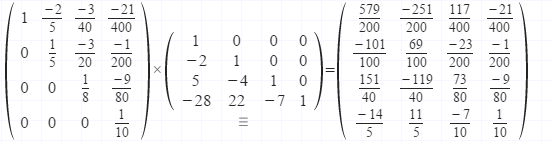
\includegraphics[scale=0.9]{1.png}

\end{document}